\documentclass[german]{article}

\usepackage[utf8]{inputenc}
\usepackage[ngerman]{babel}
\usepackage{csquotes}
\usepackage{graphicx}

\title{Eine Grenzfunktion\\ mit interessanten Eigenschaften\\[0.4em]
\large Jubiläumsvorlesung am 1.\ Oktober 2019\\
von Univ.Prof.\ em.\ Roman Schnabl\\
für den Studienjahrgang 1989 "Technische Mathematik"\\
anlässlich 30 Jahre Studienbeginn
}
\author{Wolfgang Stöcher}


\begin{document}

\maketitle

Aufbauend auf der parametrischen reellwertigen Funktionenfamilie für gerade Rechteckfunktionen mit Fläche 1 unter ihrer Kurve
\[
r_w(x) := \left\{
	\begin{array}{ll}
		\frac{1}{w}  & |x| < \frac{w}{2} \\[2pt]
		\frac{1}{2w} & |x| = \frac{w}{2} \\[2pt]
		0            & |x| > \frac{w}{2} 
	\end {array} 
	\right.
\]
wird mittels Faltung die Folge von Funktionen
\[
s_n := r_{2^0} \ast \cdots \ast r_{2^{-n}}, n \ge 1,
\]
definiert, die für $n \rightarrow \infty$ gleichmäßig gegen eine Grenzfunktion $s(x)$ konvergiert,
die wir nach ihrem Entdecker ``Schnabl-Funktion'' nennen wollen.

Die gleichmäßige Konvergenz erschließt sich z.B. aus den einfach zu zeigenden Eigenschaften
wie Geradheit ($s_n(x) = s_n(-x)$), Beschränktheit ($0 \le s_n(x) \le 1$),
Beschränktheit der Ableitung ($|s'_{n}(x)| \le s'_n(-\frac{1}{2}) = 2$) und
\[
\begin{array}{lcl}
  \left | s_{n}(x) - s_{n-1}(x) \right | & = & \left | \int_{-\infty}^{\infty} r_{2^{-n}}(t)s_{n-1}(x-t) dt - s_{n-1}(x) \right | = \\[0.4em]
                                         & = & \left | \int_{-2^{-n-1}}^{2^{-n-1}} 2^{n} s_{n-1}(x-t) dt - \int_{-2^{-n-1}}^{2^{-n-1}} 2^{n} s_{n-1}(x) dt \right | = \\[0.4em]
                                         & = & \left | 2^{n} \int_{-2^{-n-1}}^{2^{-n-1}} (s_{n-1}(x-t) - s_{n-1}(x)) dt \right | < \\[0.2em]
                                         & < & 2^{n} (2^{-n-1} - (-2^{-n-1})) \max_{|t| \le 2^{-n-1}} \left | s_{n-1}(x-t) - s_{n-1}(x) \right | < \\[0.2em]
                                         & < & 2^{n} 2^{-n} 2^{-n-1} s'_{n-1}(-\frac{1}{2}) = 2^{-n}
\end {array}
\]

Die Folgenglieder $s_n$ sind stetige Funktionen, die sich aus stückweisen Polynomfunktionen zusammensetzen.
Hier die ersten beiden Folgenglieder:
\[
s_1(x) = \int_{-\infty}^{\infty} r_1(t)r_\frac{1}{2}(x-t) dt = \left\{
	\begin{array}{ll}
		\hphantom{-}2x + \frac{3}{2}&           - \frac{3}{4} \le x \le           - \frac{1}{4} \\[2pt]
		\hphantom{-}1               &           - \frac{1}{4} \le x \le \hphantom{-}\frac{1}{4} \\[2pt]
		          - 2x + \frac{3}{2}& \hphantom{-}\frac{1}{4} \le x \le \hphantom{-}\frac{3}{4} \\[2pt]
		\hphantom{-}0               & \quad\mbox{sonst} 
	\end {array} 
	\right.
\]

\[
s_2(x) = \int_{-\infty}^{\infty} s_1(t)r_\frac{1}{4}(x-t) dt = \left\{
	\begin{array}{ll}
		\hphantom{-}4x^2 + 7x + \frac{49}{16}&           - \frac{7}{8} \le x \le           - \frac{5}{8} \\[2pt]
		\hphantom{-}2x   + \frac{3}{2}       &           - \frac{5}{8} \le x \le           - \frac{3}{8} \\[2pt]
		          - 4x^2 - x + \frac{15}{16} &           - \frac{3}{8} \le x \le           - \frac{1}{8} \\[2pt]
		\hphantom{-}1                        &           - \frac{1}{8} \le x \le \hphantom{-}\frac{1}{8} \\[2pt]
		          - 4x^2 + x + \frac{15}{16} & \hphantom{-}\frac{1}{8} \le x \le \hphantom{-}\frac{3}{8} \\[2pt]
		          - 2x   + \frac{3}{2}       & \hphantom{-}\frac{3}{8} \le x \le \hphantom{-}\frac{5}{8} \\[2pt]
		\hphantom{-}4x^2 - 7x + \frac{49}{16}& \hphantom{-}\frac{5}{8} \le x \le \hphantom{-}\frac{7}{8} \\[2pt]
		\hphantom{-}0                        & \quad\mbox{sonst} 
	\end {array} 
	\right.
\]
Die Funktionen konvergieren sehr schnell, wie man der Abbildung \ref{fig:sn} entnehmen kann.

\begin{figure}
  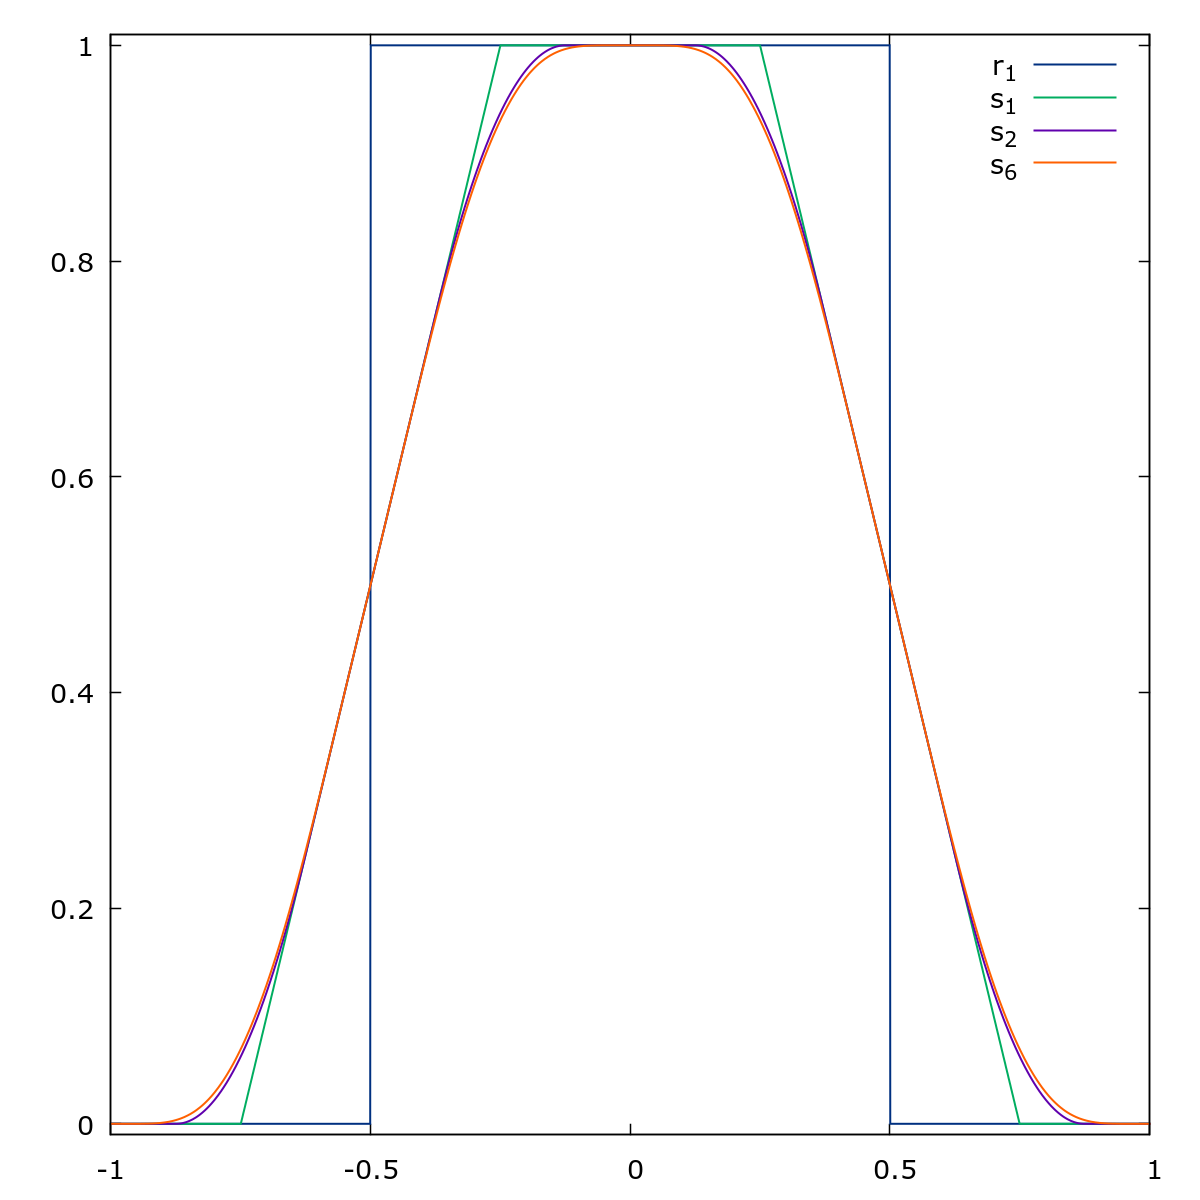
\includegraphics[width=\linewidth]{SchnablFunction.png}
  \caption{Basisfunktion $r_1$ und die Funktionen $s_1$, $s_2$ and $s_6$}
  \label{fig:sn}
\end{figure}

Die Funktionen $s_n$ haben ein paar weitere schöne Eigenschaften, die sie über die Faltung von den Basisfunktionen erben 
und die an die Grenzfunktion weiter vererbt werden:
\begin{itemize}
\item Alle Funktionswerte sind im Interval $[0,1]$. Außerhalb des Intervalls [-1,1] sind die Funktionswerte 0.
\item Die Graphen aller Funktionen laufen durch die Punkte $(\pm 1,0), (\pm \frac{1}{2},\frac{1}{2}), (0,1)$ 
      und haben dort jeweils die Ableitungen $0, \pm 2, 0$.
\item Die Funktionen sind nicht nur gerade, sondern in der Umgebung von $(\pm \frac{1}{2},\frac{1}{2})$ auch ungerade, soll heißen:
      \[ s_n(-\frac{1}{2}-t) + s_n(-\frac{1}{2}+t) = s_n(\frac{1}{2}-t) + s_n(\frac{1}{2}+t) = 1, \quad t \in [-\frac{1}{2},\frac{1}{2}]. \] 
	  Die Graphen der Funktionen $s_n$ und der Funktion $s$ über dem Interval [-1,1] bestehen also aus je 4 identischen Kurvenabschnitten.
\item Die Fläche unter jeder der Kurven ist 1.
\end{itemize}

Die Grenzfunktion hat eine zusätzliche schöne Eigenschaft: die fraktale Struktur in den Ableitungen.
Aus
\[s'_{n+1}(x) = \left\{
	\begin{array}{ll}
		\hphantom{-}2s_n(2x+1) & x<0 \\[2pt]
		          - 2s_n(2x-1) & x\ge 0
	\end {array}
\right.
\]
ergibt sich
\[\frac{s^{(k)}(x)}{2^k} = \left\{
	\begin{array}{ll}
		\hphantom{-}s^{(k-1)}(2x+1) & x<0 \\[2pt]
		          - s^{(k-1)}(2x-1) & x\ge 0
	\end {array} 
\right.
\]
In Abbildung \ref{fig:der} ist diese Eigenschaft beispielhaft an $s_6$ illustriert.

\begin{figure}
  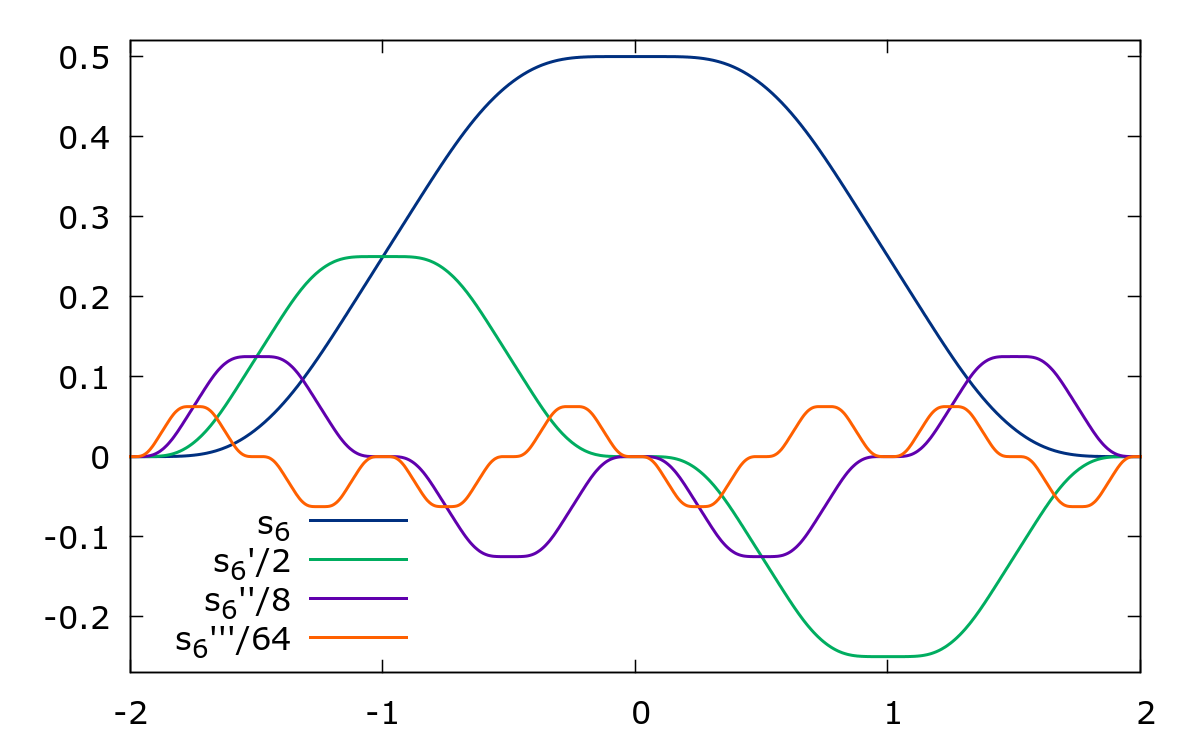
\includegraphics[width=\linewidth]{SchnablFunction_derivatives.png}
  \caption{Die Funktion $s_6$ (die der Grenzfunktion $s$ schon sehr nahe ist) und ihre ersten 3 Ableitungen (geeignet skaliert), 
  um die fraktale Struktur der Ableitungen der Grenzfunktion zu illustrieren}
  \label{fig:der}
\end{figure}

\end{document}
